\section{Methodology}
In this section, we first introduce some key notations and concepts in this work.
Then, we provide the details for each component of our proposed framework K-RagRec.

\subsection{Preliminary}


\textbf{Knowledge Graph:}
In this work, we propose to leverage external knowledge databases (i.e., KGs) to augment LLMs for recommendations.
KGs contain abundant factual knowledge in the form of a set of triples: $\mathcal{G}=\{(n,e,n') \ | \ n,n' \in N \ , \ e \in E\}$, where $N$ and $E$ denote the set of entities and relations, respectively. For example, a triple $Interstellar \ \xrightarrow{directed\_by} \ Nolan$ indicates that the movie \textit{"Interstellar"} was directed by the director \textit{"Nolan"}.

\noindent \textbf{LLM-based Recommendations:}
Let $U=\{u_1,u_2,\dots,u_n\}$ and $V=\{v_1,v_2,\dots,v_m\}$ represent the sets of users and items, where $n$ and $m$ are the sizes of users and items, respectively. 
The goal of an LLM-based recommender system is to understand users' preferences by modeling users' historical items interactions $V^{u_i}=[v^{u_i}_1, v^{u_i}_2, \cdots,v^{u_i}_{|L_{u_i}|} ]$ (\textit{e.g.}, clicks, bought, etc.), where $|L_{u_i}|$ is interaction sequence length for user $u_i$.  
Notably,  item $v_j$' side information, such as title and description, is publicly available to enhance LLM for modeling user preferences.  
In our setting, we consider asking the LLM to select user $u$'s preferred item $v$ from the candidate set $C = \{v_j\}^M_{j=1}$, where $M$ is the number of candidate items. The candidate set $C$ typically consists of one positive sample as well as $M-1$ negative samples.
Specifically, for a frozen LLM $f_{\delta}$ with parameters $\delta$, we denote an input-output sequence pair as $(Q, A)$, where $Q$ is the recommendation query/prompt, which consists of task descriptions and users' historical items. The output $A$ is the LLM's prediction. Furthermore, we introduce the concept of GNNs in appendix~\ref{appendix:gnn}.



\subsection{The Overview of Proposed Method}
As shown in Figure~\ref{fig:framework}, our proposed K-RagRec consists of five crucial components: \emph{Hop-Field Knowledge Sub-graphs for Semantic Indexing, Popularity Selective Retrieval Policy, Knowledge Sub-graphs Retrieval, Knowledge Sub-graphs Re-Ranking, and Knowledge-augmented Recommendation.} The model first performs indexing of hop-field knowledge sub-graphs within the KG. 
Following this, a popularity selective retrieval policy is implemented to determine which items should be retrieved or augmented. The model then retrieves specific sub-graphs from the knowledge vector database. 
Subsequently, the retrieved knowledge sub-graphs are re-ranked to refine the retrieval quality. Finally, the retrieved knowledge sub-graphs are utilized with the original prompt to generate recommendations.

\subsection{Hop-Field Knowledge Sub-graphs for Semantic Indexing} 
\begin{figure*}[htb]
    \centering
    \vskip -0.1in
    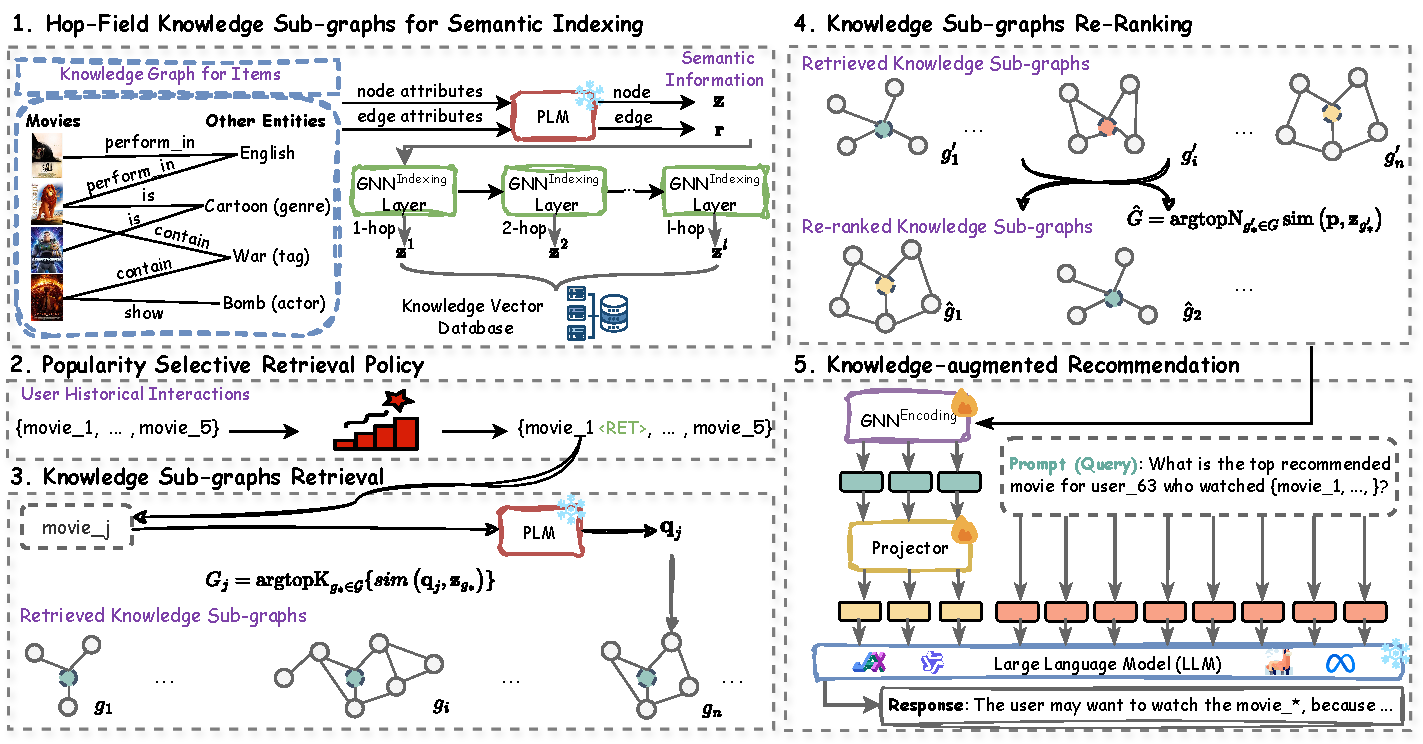
\includegraphics[width=0.95\textwidth]{figures/framework2.pdf}
    \vskip -0.1in
    \caption{The overview of the K-RagRec. 
It contains five key components: \emph{Hop-Field Knowledge Sub-graphs for Semantic Indexing, Popularity Selective Retrieval Policy, Knowledge Sub-graphs Retrieval, Knowledge Sub-graphs Re-Ranking, and Knowledge-augmented Recommendation.}
    }
    \label{fig:framework}
    \vskip -0.2in
\end{figure*}


Typically, retrieving knowledge from KG chunks the KG into nodes~\citep{he2024g} or triplets~\citep{luo2023reasoning} and only retrieves content locally around the target entity in the KG.
However, these methods just naively retrieve the first-order neighbors of an entity (i.e., item), which makes it difficult to capture these higher-order neighborhood effects among entities/items in the recommendation process. 
Therefore, to effectively retrieve knowledge from the KG, we propose performing semantic indexing on hop-field knowledge sub-graphs, which can flexibly chunk KGs and provide a comprehensive view of a node's neighborhood in KG.
As illustrated in Figure~\ref{fig:framework} component 1, we first introduce a pre-trained language model (PLM), such as SentenseBert~\citep{reimers2019sentence},  to capture the semantic information for node $n_o$ as follows:
\begin{equation}
\setlength{\abovedisplayskip}{3pt}
\setlength{\belowdisplayskip}{3pt}
\textbf{z}_{n_o}=\text{PLM}(x_{n_o})\in {R}^d,
\end{equation}
where $d$ is the dimension of the output representation. Similarly, we also capture the semantic information for edge/relation $e_o$ in KG:
\begin{equation}
\setlength{\abovedisplayskip}{3pt}
\setlength{\belowdisplayskip}{3pt}
\textbf{r}_{e_o}=\text{PLM}(x_{e_o})\in {R}^d,
\end{equation}
where $x_{n_o}$ and $x_{e_o}$ are the text attributes (e.g., item's title and descriptions) of node $n_o$ and edge/relation $e_o$, respectively.

To retrieve nuanced knowledge of both coarse and fine graph structures from KG, we introduce a GNN (i.e., $\text{GNN}_{\phi_1}^{\text{Indexing}} (\cdot)$ with parameters $\phi_1$) to aggregate information from neighbors for entities, where the $l_{th}$-hop embedding $\textbf{z}_{n_o}^{(l)}$ of a central entity $n_o$ can be defined by:
\begin{small}
\begin{equation}
\setlength{\abovedisplayskip}{3pt}
\setlength{\belowdisplayskip}{3pt}
% \begin{aligned} 
\textbf{z}_{n_o}^{l} = \text{GNN}_{\phi_1}^{\text{Indexing}} (\{\textbf{z}_{n_m}^{(l-1)}, \textbf{r}_{e_{<o, m>}}^{(l-1)}: \\
~ n_m \in \mathcal{N}(n_o)   \}),
% \end{aligned}
\end{equation}
\end{small}
where $\mathcal{N}(n_o)$ is the set of neighbours of node $n_o$, 
and $e_{<o, m>}$ is the edge between node $n_o$ and $n_m$.
For each entity, its $l$-hop representation can be seen as a knowledge sub-graph representation containing the $l$-hop neighbors of itself. 
Therefore, we can express the knowledge sub-graph representation of $g_o \in \mathcal{G}$ as $\textbf{z}_{g_o}$, where $\mathcal{G}$ is the set containing all the knowledge sub-graphs. For each sub-graph, we store its representation in a \emph{knowledge vector database}. 






 \subsection{Popularity Selective Retrieval Policy}
Although RAG can augment the LLM for modeling user preferences with retrieved knowledge, retrieving each item can cost a significant amount of retrieval time, which can severely degrade the user experience and cause user churn.
Meanwhile, most users’ online behaviours in recommender systems are following the power law distribution~\citep{abdollahpouri2017controlling,celma2008new} in which a small proportion (e.g., less than 20\%) of items (i.e., popular items) often account for a large proportion of users’ online behaviours (e.g., more than 80\%), while cold-start items have a few interactions from users.
Therefore, most models tend to keep rich knowledge of popular items, resulting in an inferior performance for cold-start items~\citep{zhao2023popularity}. 
To this end, we design a popularity selective retrieval policy to determine whether an item needs to be augmented from KG based on its popularity (e.g., sales volume and page view). 
Particularly, the item is retrieved if its popularity is less than the pre-defined threshold $p$, otherwise not. 
By incorporating this strategy, the retrieval time in K-RagRec can be significantly reduced to achieve more efficient retrieval. 


 \subsection{Knowledge Sub-graphs Retrieval} 
Given the query for knowledge sub-graphs retrieval, we adopt the same PLM as the first indexing step to ensure that the query is in the consistent embedding space as the knowledge sub-graph representation. 
We define the text attribute (e.g., item's title and descriptions) $x_{q_j}$ of the item $v_j$ that needs to be retrieved as the query and obtain its semantic information $\textbf{q}_j$ as: 
\begin{equation}
\setlength{\abovedisplayskip}{2pt}
\setlength{\belowdisplayskip}{2pt}
\textbf{q}_j=\text{PLM}(x_{q_j})\in {R}^d.
\end{equation}


Next, we retrieve the top-$K$ most similar sub-graphs $G_j=\{g'_1, ..., g'_K\}$ from  $\mathcal{G}$ for item $v_j$:  
\begin{equation}
\setlength{\abovedisplayskip}{3pt}
\setlength{\belowdisplayskip}{3pt}
G_{j} = \operatorname{argtopK}_{g_* \in \mathcal{G}} \text{sim} \left(\textbf{q}_j, \textbf{z}_{g_*} \right),
\end{equation}
where  ${\text{sim}(\cdot, \cdot)}$ is a similarity metric for measuring the similarity between the query representation $\textbf{q}_j$ and knowledge sub-graph ${g_*}$'s representation $\textbf{z}_{g_*}$  in knowledge vector database. 
Finally,  the retrieved knowledge sub-graphs for items required to be retrieved from user ${u_i}$'s historical interactions $V^{u_i}$ will be used to form a knowledge sub-graph set $G$.


\subsection{Knowledge Sub-graphs Re-Ranking} 
To refine the quality of retrieval for enhancing recommendation performance, the next crucial step is knowledge sub-graphs re-ranking.
Feeding all retrieved knowledge sub-graphs $g' \in G$ directly into LLM can lead to information overload if the user ${u_i}$ has a long historical interaction list towards items.
Therefore, we execute re-ranking to shorten the retrieved knowledge sub-graphs and ensure the most relevant knowledge sub-graphs are prioritized at the top of the prompt. 
Specifically, we adopt the recommendation prompt as a query for re-ranking, which consists of \textbf{task descriptions} and \textbf{users’ historical items}.
For example, this recommendation prompt can be \textit{"What is the top recommended movie for the user who watched \{Matrix, ..., Iron Man\}?"}. 
For consistency, we adopt the same PLM to capture the semantic information of the above prompt as $\textbf{p}$, and re-rank the knowledge sub-graphs in $G$ to obtain a  Top-$N$ knowledge sub-graphs set $\hat{G}$: 
\begin{equation}
\setlength{\abovedisplayskip}{3pt}
\setlength{\belowdisplayskip}{3pt}
\hat{G}=\operatorname{argtopN}_{g_*' \in G} \text{sim} \left(\textbf{p}, \textbf{z}_{g_*'} \right).
\end{equation}



 \subsection{Knowledge-augmented Recommendation}
To facilitate the LLM's better understanding of the structure of retrieved knowledge sub-graphs and to avoid long contexts, we further integrate another  GNN encoder $\text{GNN}^{\text{Encoding}}_{\phi_2}$ with parameter ${\phi_2}$ to enhance the representation learning of structural information:
\begin{equation}
\setlength{\abovedisplayskip}{3pt}
\setlength{\belowdisplayskip}{3pt}
\textbf{h}_{\hat{g_*}}=\text{GNN}^{\text{Encoding}}_{\phi_2}(\{\hat{g_*}: \hat{g}_*\in \hat{G}\}).
\end{equation}



An MLP projector $\text{MLP}_{\theta}$ with parameter $\theta$ is further introduced to shift to mapping all sub-graphs embedding in $\hat{G}$ into the LLM embedding space:

% \vspace{-0.1in}
\begin{equation}
\setlength{\abovedisplayskip}{2pt}
\setlength{\belowdisplayskip}{2pt}
\hat{\textbf{h}}_{\hat{G}}= \text{MLP}_{\theta}([\textbf{h}_{\hat{g_1}};...;\textbf{h}_{\hat{g_N}}]),
\end{equation}
where $[.; .]$ represents the concatenation operation. 
The extracted knowledge sub-graphs embedding $\hat{\textbf{h}}_{\hat{G}}$ as the soft prompt is then appended before the input token embedding in LLM. 


\subsection{Optimization for K-RagRec} 
The training process can be broadly considered as soft prompt tuning, where the retrieved knowledge sub-graphs are a series of soft graph prompts.
Formally, the generation process can be expressed as follows:
\begin{small} 
\begin{equation}
\setlength{\abovedisplayskip}{3pt}
\setlength{\belowdisplayskip}{3pt}
% \begin{aligned} 
p_{\delta, \theta, \phi_1, \phi_2}(Y \mid \hat{G}, x_q) =
\prod_{k=1}^r p_{\delta, \theta, \phi_1, \phi_2}(y_k \mid y_{<k}, \hat{\textbf{h}}_{\hat{G}}, x_q).
% \end{aligned}
\end{equation}
\end{small}

Therefore, instead of fine-tuning the LLM model extensively, we only learn parameters of two GNNs (i.e., $\text{GNN}_{\phi_1}^{\text{Indexing}}$, $\text{GNN}_{\phi_2}^{\text{Encoding}}$) and projector  $\text{MLP}_\theta$, while parameters $\delta$ of LLM backbone are frozen. We update the parameters $\phi_1$, $\phi_2$ and $\theta$ through the Cross-Entropy Loss $\mathcal{L}(Y,A)$, where $Y$ is the ground-truth and $A$ is LLM's prediction.
